\chapter{BRDF models used in road surface}
\label{ch: brdf-models}

Reflectance models are typically introduced in order to achieve low-parameter representation of the BRDF measurements acquired from road surfaces~\cite{2010_Roser}.
Many road surfaces exhibit non-diffuse characteristics, simplified Lambertian assumptions are insufficient for accurate optical predictions.
This is especially true for surfaces that include specular peaks due to polishing or for materials that have retro-reflective properties, such as in tunnel markings or retro-reflective coatings~\cite{2019_Iacomussi}.
To address these complexities, this chapter explores a range of reflectance models utilized for characterizing the BRDF of various road materials, such as concrete, sand, aggregates.

%%%%%%%%%%%%%%%%%%%%%%%%%%%%%%%%
\section{Microfacet-based BRDF models}

\begin{figure}
    \centering
    \subfigure[Shadowing]{
        \centering
        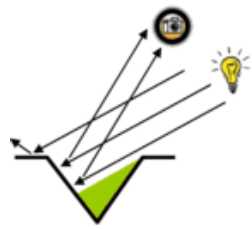
\includegraphics[width=0.3\linewidth]{./figures/brdf-models-of-roads/shadowing.png}
        \label{fig:shadowing}
    }
    \subfigure[Masking]{
        \centering
        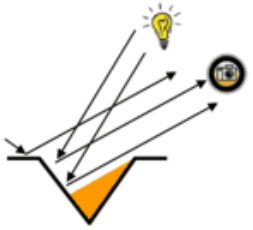
\includegraphics[width=0.3\linewidth]{./figures/brdf-models-of-roads/masking.png}
        \label{fig:masking}
    }
    \subfigure[Interreflection]{
        \centering
        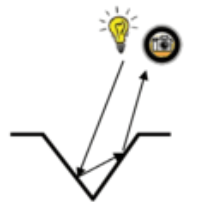
\includegraphics[width=0.25\linewidth]{./figures/brdf-models-of-roads/inter-reflection.png}
        \label{fig:inter-reflection}
    }
    \caption{Physical phenomena in microfacets}
\end{figure}

This section introduces two widely used reflectance models used in road surface: Oren-Nayar (ON) BRDF for describing diffuse reflection and Torrance Sparrow (TS) / Cook-Torrance (CT) BRDF for describing specular reflection.
Both are based on microfacet theory which represents the surface of a collection of small surfaces.
In graphics community, microfacet theory was used to derive physically based BRDF~\cite{2014_Heitz}, and typically accounts for complex geometric and radiometric phenomena:
\begin{itemize}
    \item shadowing, where the facet is only partially illuminated because the adjacent facet casts a shadow on it, as seen in Fig~\ref{fig:shadowing};
    \item masking, where the facet is only partially visible to the camera because its adjacent facet occludes it, as seen in Fig~\ref{fig:masking}.
\end{itemize}
Their impacts are described using shadowing function and masking function, respectively.
A meaningful microfacet model is described by a distribution of normals, which models how the microfacets are statistically oriented, and a microfacet profile, which models how the microfacets are organized on the microfacet.
Mathematically, the general microfacet-based BRDF expression is following as:
% \begin{equation}
%     \label{eq_brdf_microfacet}
%     f_r(\overrightarrow{\omega_i}, \overrightarrow{\omega_r}) = \frac{1}{\cos(\theta_r) \cos(\theta_i)}%
%     \int_\Omega f_{r(M)}(\overrightarrow{\omega_i}, \overrightarrow{\omega_r}, \overrightarrow{\omega_m})%
%     (\overrightarrow{\omega_r} \cdot \overrightarrow{\omega_m}) (\overrightarrow{\omega_i} \cdot \overrightarrow{\omega_m})%
%     G(\overrightarrow{\omega_i}, \overrightarrow{\omega_r}, \overrightarrow{\omega_m})%
%     D(\overrightarrow{\omega_m})\mathrm{d} \overrightarrow{\omega_m},
% \end{equation}


% where:
% \begin{itemize}
% \item $\overrightarrow{\omega_i}, \overrightarrow{\omega_r}, \overrightarrow{\omega_m}$ are the directions of the incident light, detection and the normal of the microfacet;
% \item $f_{r(M)}(\overrightarrow{\omega_i}, \overrightarrow{\omega_r}, \overrightarrow{\omega_m})$ is the BRDF of each microfacet;
% \item $D(\overrightarrow{\omega_m})$ represents the distribution of the normals of the microfacets;
% \item $G(\overrightarrow{\omega_i}, \overrightarrow{\omega_r}, \overrightarrow{\omega_m})$ is geometric attenuation function, combining masking $G_1$ and shadowing $G_2$ function.
% It gives the fraction of microfacets with normal $\overrightarrow{\omega_m}$ that are visible along the reflected direction $\overrightarrow{\omega_r}$, depending on the microfacet profile (e.g. V-cavity microfacet profile and smith microfacet profile) and the distribution of the microfacet's normal~\cite{2014_Heitz}.
% The masking $G_1$ and shadowing $G_2$ function are formalized by the following equations:
% \begin{equation}
%     \begin{array}{lll}
%         \label{eq_masking_shadowing}
%         \cos\theta_r & = & \displaystyle{
%             \int_{\Omega} G_1(\overrightarrow{\omega_r}, \overrightarrow{\omega_m}) (\overrightarrow{\omega_r} \cdot \overrightarrow{\omega_m}) D(\overrightarrow{\omega_m}) \mathrm{d} \overrightarrow{\omega_m}
%         }                                                                                                                                                                                                                                       \\ \\
%         \cos\theta_i & = & \displaystyle{\int_{\Omega} G_2(\overrightarrow{\omega_i}, \overrightarrow{\omega_m}) (\overrightarrow{\omega_i} \cdot \overrightarrow{\omega_m}) D(\overrightarrow{\omega_m}) \mathrm{d} \overrightarrow{\omega_m}}
%     \end{array}
% \end{equation}


\begin{equation}
    \label{eq_brdf_microfacet}
    \begin{array}{ll}
        f_r(\lambda, \theta_i, \varphi_i, \theta_r, \varphi_r) = & \frac{1}{\cos(\theta_r) \cos(\theta_i)}            %
        \int_{0}^{\pi /2} \int_{0}^{2\pi}%
        f_{r(M)}(\lambda, \theta_i, \varphi_i, \theta_r, \varphi_r, \theta_m, \varphi_m)                              \\
                                                                 & \times (\cos\theta_r^\prime) (\cos\theta_i^\prime) %
        G(\theta_i, \varphi_i, \theta_r, \varphi_r, \theta_m, \varphi_m)%
        D(\theta_m, \varphi_m)\mathrm{d} \theta_m \mathrm{d} \varphi_m,
    \end{array}
\end{equation}

where:
\begin{itemize}
    \item $\theta_i, \varphi_i$ are the zenith and azimuth angles of the unit incident direction $\overrightarrow{\omega_i}$,

    \item $\theta_r, \varphi_r$ are the zenith and azimuth angles of the unit reflected direction $\overrightarrow{\omega_r}$,

    \item $\theta_m, \varphi_m$ are the zenith and azimuth angles of the unit normal of the microfacet $\overrightarrow{\omega_m}$,

    \item $\theta_i^\prime$ is the angle between the incident direction $\overrightarrow{\omega_i}$ and the normal of the microfacet $\overrightarrow{\omega_m}$,

    \item $\theta_r^\prime$ is the angle between the reflected direction $\overrightarrow{\omega_r}$ and the normal of the microfacet $\overrightarrow{\omega_m}$,

    \item $f_{r(M)}(\lambda, \theta_i, \varphi_i, \theta_r, \varphi_r, \theta_m, \varphi_m)$ is the BRDF of each microfacet,

    \item $D(\theta_m, \varphi_m)$ represents the distribution of the normals of the microfacets;

    \item $G(\theta_i, \varphi_i, \theta_r, \varphi_r, \theta_m, \varphi_m)$ is geometric attenuation function, combining masking $G_1$ and shadowing $G_2$ function.
          It gives the fraction of microfacets with normal $\overrightarrow{\omega_m}$ that are visible along the reflected direction $\overrightarrow{\omega_r}$, depending on the microfacet profile (e.g. V-cavity microfacet profile and smith microfacet profile) and the distribution of the microfacet's normal~\cite{2014_Heitz}.
          The masking $G_1$ and shadowing $G_2$ function are formalized by the following equations:
          \begin{equation}
              \begin{array}{lll}
                  \label{eq_masking_shadowing}
                  \cos\theta_r & = & \displaystyle{
                      \int_{0}^{\pi/2} \int_{0}^{2\pi}%
                      G_1(\theta_r, \varphi_r, \theta_m, \varphi_m) %
                      (\cos\theta_r^\prime)%
                      D(\theta_m, \varphi_m) \mathrm{d} \mathrm{d} \theta_m \mathrm{d} \varphi_m%
                  }                                                                 \\ \\
                  \cos\theta_i & = & \displaystyle{\int_{0}^{\pi/2} \int_{0}^{2\pi} % 
                      G_2(\theta_i, \varphi_i, \theta_m, \varphi_m)% 
                      (\cos\theta_i^\prime)% 
                      D(\theta_m, \varphi_m) \mathrm{d} \theta_m \mathrm{d} \varphi_m}
              \end{array}
          \end{equation}

\end{itemize}

%%%%%%%%%%%%%%%%%%%%%%%%%%%%%%%%%%%%%%%%%%%%%%
\subsection{Oren-Nayar BRDF}\label{subsec: oren-nayar-model}

The Oren-Nayar BRDF is widely used for modelling diffuse reflections from rough surfaces, as it provides a more realistic representation of light behavior compared to simpler Lambertian model~\cite{1995_Oren,1995_Oren,2010_Roser}.
This model was first proposed in 1994~\cite{1995_Oren} by Oren and Nayar, based on microfacet theory adapting V-cavity microfacet profile.
More precisely, the surface is assumed as a collection of long, symmetric v-shaped cavities with equal length, each containing two opposing planar facets.
This implies that each V-cavity has the two symmetric normals $\overrightarrow{\omega_m}$ and $\overrightarrow{\omega_m^\prime}$, leading to the following distribution of normals of each microfacet $D(\theta, \varphi)$:
% \[
%     D(\overrightarrow{\omega}) = \frac{1}{2} \frac{\delta(\overrightarrow{\omega} - \overrightarrow{\omega_m})}{\overrightarrow{\omega_m} \cdot \overrightarrow{n}}%
%     + \frac{1}{2} \frac{\delta(\overrightarrow{\omega} - \overrightarrow{\omega_m^\prime})}{\overrightarrow{\omega_m^\prime} \cdot \overrightarrow{n}}
% \]
\[
    D(\theta, \varphi) = \frac{1}{2} \frac{\delta(\overrightarrow{\omega} - \overrightarrow{\omega_m})}{\cos \theta_m}%
    + \frac{1}{2} \frac{\delta(\overrightarrow{\omega} - \overrightarrow{\omega_m^\prime})}{\cos\theta_m^\prime}
\]
Where $\theta_m, \theta_m^\prime$ are zenith angles of the normals of the microfacet $\overrightarrow{\omega_m}, \overrightarrow{\omega_m^\prime}$.

The masking or shadowing term can be derived according to Equation\eqref{eq_masking_shadowing} considering if there is no or one backfacing normal direction:
% \[
%     \begin{array}{lll}
%         G_1(\overrightarrow{\omega_r}, \overrightarrow{\omega_m}) & = & \displaystyle{\min\left(1,                                                                                            %
%         2\frac{(\overrightarrow{\omega_m} \cdot \overrightarrow{n})(\overrightarrow{\omega_r} \cdot \overrightarrow{n})}{(\overrightarrow{\omega_r} \cdot \overrightarrow{\omega_m})}\right)} \\ \\
%         G_2(\overrightarrow{\omega_i}, \overrightarrow{\omega_m}) & = & \displaystyle{\min\left(1,                                                                                            %
%             2\frac{(\overrightarrow{\omega_m} \cdot \overrightarrow{n})(\overrightarrow{\omega_i} \cdot \overrightarrow{n})}{(\overrightarrow{\omega_i} \cdot \overrightarrow{\omega_m})}\right)}
%     \end{array}
% \]
\[
    \begin{array}{lll}
        G_1(\theta_r, \varphi_r, \theta_m, \varphi_m) & = & \displaystyle{\min\left(1, %
        2\frac{(\cos\theta_m)(\cos\theta_r)}{(\cos\theta_r^\prime)}\right)}            \\ \\
        G_2(\theta_i, \varphi_i, \theta_m, \varphi_m) & = & \displaystyle{\min\left(1, %
            2\frac{(\cos\theta_m)(\cos\theta_m)}{(\cos\theta_i^\prime)}\right)}
    \end{array}
\]

Considering both masking and shadowing,  the term $G(\theta_i, \varphi_i, \theta_r, \varphi_r, \theta_m, \varphi_m)$ can be derived as:
% \begin{equation}
%     \label{eq_g_v_gaussian}
%     G(\overrightarrow{\omega_i}, \overrightarrow{\omega_r}, \overrightarrow{\omega_m}) = \min\left(1, %
%     2\frac{(\overrightarrow{\omega_m} \cdot \overrightarrow{n})(\overrightarrow{\omega_r} \cdot \overrightarrow{n})}{(\overrightarrow{\omega_r} \cdot \overrightarrow{\omega_m})},%
%     2\frac{(\overrightarrow{\omega_m} \cdot \overrightarrow{n})(\overrightarrow{\omega_i} \cdot \overrightarrow{n})}{(\overrightarrow{\omega_i} \cdot \overrightarrow{\omega_m})}\right)
% \end{equation}
\begin{equation}
    \label{eq_g_v_gaussian}
    G(\theta_i, \varphi_i, \theta_r, \varphi_r, \theta_m, \varphi_m) = \min\left(
    1, %
    2\frac{(\cos\theta_m)(\cos\theta_r)}{(\cos\theta_r^\prime)},%
    2\frac{(\cos\theta_m)(\cos\theta_m)}{(\cos\theta_i^\prime)}
    \right)
\end{equation}
The distribution of the normals of all microfacets is described using a spherical gaussian distribution with a mean value of zero and a standard deviation $\alpha$, which serves as a roughness parameter:
% \begin{equation}
%     \label{eq_gaussian}
%     D(\overrightarrow{\omega_m}) = c e^{-\frac{\theta_m^2}{2\alpha^2}},
% \end{equation}
\begin{equation}
    \label{eq_gaussian}
    D_{gaussian}(\theta_m) = c e^{-\frac{\theta_m^2}{2\alpha^2}},
\end{equation}
where the normalization constant $c$ is:
\[
    c = \frac{1}{\displaystyle{\int_{\varphi_m=0}^{2\pi} \int_{\theta_m}^{\frac{\pi}{2}} e^{-\frac{\theta_m^2}{2\alpha^2}}\sin\theta_m \mathrm{d}\theta_m \mathrm{d}\varphi_m}}
\]
Besides, the facets are assumed to exhibit diffuse reflection, implying the BRDF of each microfacet $f_{r(M)}$ is defined as shown in Equation~\eqref{eq_Lambertian}.
By substituting $f_{r(M)}$ from Equation\eqref{eq_Lambertian} , $G$ from Equation\eqref{eq_g_v_gaussian} and $D$ from Equation\eqref{eq_gaussian} into Equation\eqref{eq_brdf_microfacet}, the reflectance model is obtained.
However, the resulting integral can not be easily evaluated.
Therefore, Oren and Nayar provided an approximation by using a identified basis function and conducting a large amounts of numerical simulations to evaluate this integral.
The approximated expression of directly reflected part is following as:
\[
    \begin{array}{ll}
        f^{dir}_{r}(\lambda, \theta_i, \theta_r, \varphi) = & \frac{\rho_d}{\pi}[ C_1(\alpha) + C_2(\theta_1, \theta_2, \varphi, \alpha)\cos(\varphi) \tan(\theta_2)              \\
                                                            & + C_3(\theta_1, \theta_2, \alpha) \left(1 - |\cos(\varphi)| \right) \tan\left(\frac{\theta_1 + \theta_2}{2}\right)]
    \end{array}
\]
where:
\begin{itemize}
    \item $\rho_d$ is the albedo of each facet;
    \item $\varphi = |\varphi_i - \varphi_r|$ is the relative azimuth angle;
    \item $\theta_1 = \max(\theta_i, \theta_r)$ is the maximum zenith angle between $\theta_i$ and $\theta_r$;
    \item $\theta_2 = \min(\theta_i, \theta_r)$ is the minimum zenith angles between $\theta_i$ and $\theta_r$;
    \item $\alpha$ (in radians) is a parameter for the surface roughness, which is gaussian standard deviation in angles of the microfacets normal
    \item $C_1, C_2, C_3$ are constant:
          \[
              \begin{array}{lll}
                  C_1(\alpha)                              & = & 1  - 0.5\frac{\alpha^2}{\alpha^2 + 0.33}                                                                                                      \\ \\
                  C_2(\theta_1, \theta_2, \varphi, \alpha) & = & \begin{cases}
                                                                     0.45 \frac{\alpha^2}{\alpha^2 + 0.09}\sin(\theta_1),                                                     & \mbox{if $\cos(\varphi) \ge 0$} \\ \\
                                                                     0.45 \frac{\alpha^2}{\alpha^2 + 0.09}\left(\sin(\theta_1) - \left(\frac{2\theta_2}{\pi}\right)^3\right), & \mbox{otherwise}
                                                                 \end{cases} \\ \\
                  C_3(\theta_1, \theta_2, \alpha)          & = & 0.125 \left(\frac{\alpha^2}{\alpha^2 + 0.09}\right) \left(\frac{4\theta_1 \theta_2}{\pi^2}\right)^2
              \end{array}
          \]
\end{itemize}
In a V-cavity microfacet, apart from the shadowing and masking effects described in microfacet theory, light rays may also bounce between adjacent facets, as seen in Fig~\ref{fig:inter-reflection}.
This phenomenon is referred to as inter-reflections.
In the case of Lambertian surfaces, the energy in an incident light diminishes rapidly with each inter-reflection bounce~\cite{1995_Oren}.
Accordingly, Oren and Nayar consider only two bounces inter-reflections and neglect the subsequent bounces.
Similar to direct illumination component, the multiple inter-reflections part is approximated as:
\[
    f^{ms}_{r}(\lambda, \theta_i, \theta_r, \varphi) = 0.17 \frac{\rho_d^2}{\pi} \frac{\alpha^2}{\alpha^2 + 0.13} \left(1 - \frac{4\theta^2_2}{\pi^2} \cos(\varphi)\right)
\]
Combing the directly reflected part and the multiple inter-reflections part, the complete expression of the ON BRDF is:
\begin{equation}
    \label{eq_brdf_ON}
    f_{r(ON)}(\lambda, \theta_i, \theta_r, \varphi)   = f^{dir}_{r}(\lambda, \theta_i, \theta_r, \varphi) + f^{ms}_{r}(\lambda, \theta_i, \theta_r, \varphi)
\end{equation}
Notice that this model reduces to Lambertian BRDF when the roughness $\alpha=0$.

This model has been applied to road materials, such as plaster and white sand in \cite{1995_Oren}, where it provides a good fit with experimental measurements, with the fitting parameters $\rho_d = 0.9, \alpha = 30^\circ$ for the former and $\rho_d = 0.8, \alpha = 35^\circ$ for the latter.

%%%%%%%%%%%%%%%%%%%%%%%%%%%%%%%%%%%%%
\subsection{Torrance-Sparrow / Cook Torrance BRDF}
\label{subsec:brdf-cook-torrance}

The specular reflection model of rough surfaces first introduced by Torrance and Sparrow in 1967 has gained widespread attention~\cite{1995_Oren,2000_Meister,2010_Roser,2023_Lucas,2024_Lucas}.
This model is also based on microfacet theory, where each facet is assumed to exhibit specular reflection, corresponding to Equation~\eqref{eq_specular}.
Consequently, the BRDF of each microfacet $f_{r(M)}$ presented in Equation\eqref{eq_brdf_microfacet} can be derived as:
% \[
%     \begin{array}{lll}
%         f_{r(M)}(\overrightarrow{\omega_i}, \overrightarrow{\omega_r}, \overrightarrow{\omega_m}) & = & \displaystyle{\left|\frac{\partial \overrightarrow{\omega_h}}{\partial \overrightarrow{\omega_i}} \right| % 
%             \frac{F_r(\overrightarrow{\omega_i}, \overrightarrow{\omega_h}) \delta(\overrightarrow{\omega_m} - \overrightarrow{\omega_h})}%
%             {\left| \overrightarrow{\omega_i} \cdot \overrightarrow{\omega_h} \right|}
%         }                                                                                                                                                                                                         \\ \\
%                                                                                                   & = & \displaystyle{
%             \frac{F_r(\overrightarrow{\omega_i}, \overrightarrow{\omega_h}) \delta(\overrightarrow{\omega_m} - \overrightarrow{\omega_h})}%
%             {4\left| \overrightarrow{\omega_i} \cdot \overrightarrow{\omega_h} \right|^2}
%         },
%     \end{array}
% \]
\[
    \begin{array}{lll}
        f_{r(M)}(\lambda, \theta_i, \varphi_i, \theta_r, \varphi_r, \theta_m, \varphi_m) & = & \displaystyle{\left|\frac{\partial \overrightarrow{\omega_h}}{\partial \overrightarrow{\omega_i}} \right| % 
            \frac{F_r(\lambda, \theta_i^\prime)%
                \delta(\overrightarrow{\omega_m} - \overrightarrow{\omega_h})}%
            {\left| \cos\theta_i^\prime \right|}
        }                                                                                                                                                                                                \\ \\
                                                                                         & = & \displaystyle{
            \frac{F_r(\lambda, \theta_i^\prime)% 
                \delta(\overrightarrow{\omega_m} - \overrightarrow{\omega_h})}%
            {4\left| \cos\theta_i^\prime \right|^2}
        },
    \end{array}
\]


where $\overrightarrow{\omega_h}$ is unit halfway vector, and defined as:
\begin{equation}
    \label{eq_half-vector}
    \begin{array}{lll}
        \overrightarrow{\omega_h} & = & \frac{\overrightarrow{\omega_i} + \overrightarrow{\omega_r}}{\left|\overrightarrow{\omega_i} + \overrightarrow{\omega_r}\right|} = (x_h, y_h, z_h) \\
        x_h                       & = & \frac{x_i + x_r}{\sqrt{(x_i + x_r)^2 + (y_i + y_r)^2 + (z_i + z_r)^2}}                                                                             \\
        y_h                       & = & \frac{y_i + y_r}{\sqrt{(x_i + x_r)^2 + (y_i + y_r)^2 + (z_i + z_r)^2}}                                                                             \\
        z_h                       & = & \frac{z_i + z_r}{\sqrt{(x_i + x_r)^2 + (y_i + y_r)^2 + (z_i + z_r)^2}}
    \end{array}
\end{equation}
The term $\left|\frac{\partial \overrightarrow{\omega_h}}{\partial \overrightarrow{\omega_i}} \right|$ is the jacobian of the reflection transformation~\cite{2007_Walter, 2014_Heitz}:
\[
    \left|\frac{\partial \overrightarrow{\omega_h}}{\partial \overrightarrow{\omega_i}} \right|
    = \frac{1}{4\left|\overrightarrow{\omega_i} \cdot \overrightarrow{\omega_h}\right|}%
    = \frac{1}{4\left|\cos\theta_i^\prime\right|}
\]
Putting this $f_{r(M)}$ into Equation\eqref{eq_brdf_microfacet}, we can replace the integral by the integrand evaluated at $\overrightarrow{\omega_m} = \overrightarrow{\omega_h}$ according to the delta dirac function $\delta(\overrightarrow{\omega_m} - \overrightarrow{\omega_h})$.
Thanks to $\overrightarrow{\omega_r}\cdot \overrightarrow{\omega_h} = \overrightarrow{\omega_i}\cdot \overrightarrow{\omega_h}$, we arrive the final expression of TS BRDF:
% \begin{equation}
%     \label{eq_brdf_TS}
%     f_{r(TS)}(\theta_i, \varphi_i, \theta_r, \varphi_r) = \frac{F_r(\overrightarrow{\omega_i}, \overrightarrow{\omega_h})% 
%         G(\overrightarrow{\omega_i}, \overrightarrow{\omega_r}, \overrightarrow{\omega_h})%
%         D(\overrightarrow{\omega_h})}%
%     {4 \cos\theta_i \cos\theta_r}
% \end{equation}
\begin{equation}
    \label{eq_brdf_TS}
    f_{r(TS)}(\theta_i, \varphi_i, \theta_r, \varphi_r) = \frac{F_r(\lambda, \theta_i^\prime)% 
        G(\theta_i, \varphi_i, \theta_r, \varphi_r,\theta_h, \varphi_h)%
        D(\theta_h)}%
    {4 \cos\theta_i \cos\theta_r}
\end{equation}
Notice that inter-reflections are not taken into account in this model.


It is known that the geometric attention function $G$ given in Equation~\eqref{eq_brdf_microfacet} is dependent of microfacet profile.
Two widely used microfacet profiles in this model are introduced: V-cavity and smith.

\begin{itemize}
    \item \textbf{V-cavity microfacet profile}

          The original formulation of Torrance-Sparrow (TS) model adapted the former profile~\cite{1967_Torrance,2000_Meister}.
          Similar to the microfacet profile used in ON model, it represents the surface as a collection of symmetric V-cavity microfacet, leading to the same $G$ function as Equation~\eqref{eq_g_v_gaussian}.
          The probability distribution of the microfacets normals $D(\theta_h)$ is often described by zero-mean Gaussian distribution function~\cite{2000_Meister,2010_Roser}, as given in Equation~\eqref{eq_gaussian}.
          Later, Cook and Torrance introduced this reflectance model to computer graphics, replacing the Gaussian function with the Beckmann distribution function~\cite{1982_Cook, 2014_Heitz}, which is derived from it:
          \begin{equation}
              \label{eq_Beckmann}
              D_{Beckmann}(\theta_h) = \frac{\chi^{+}(\cos\theta_h)}{\pi \alpha^2 \cos^4(\theta_h)}\exp\left(-\frac{\tan^2(\theta_h)}{\alpha^2}\right)
          \end{equation}
          Where the step function $\chi^{+}(\cos\theta_h)$ is the binary discard of backfacing microfacet:
          \begin{equation}
              \label{eq_step_func}
              \chi^{+}(\cos\theta_h) = \begin{cases}
                  1, & \mbox{if $\cos\theta_h > 0$} \\
                  0, & \mbox{else}
              \end{cases}
          \end{equation}
          Unlike the Gaussian model, the Beckmann distribution gives the absolute magnitude of reflectance without introducing arbitrary constants.
          However, it is more computationally expensive.


    \item \textbf{Smith microfacet profile}

          Building on Cook-Torrance (CT) reflectance model, the Smith microfacet profile was introduced into it later~\cite{2014_Heitz}.
          This profile represents more realistic surface but is more complicated, as it assumes that the microfacets are not auto-correlated.
          More precisely, it represents a random set of microfacets instead of a continuous surface, where the heights and normals of the microfacets are independent random variables~\cite{2014_Heitz}.
          A commonly used form of smith joint height-correlated masking-shadowing function is given as:
          %   \begin{equation}
          %       \label{eq_g_smith}
          %       G(\overrightarrow{\omega_i}, \overrightarrow{\omega_r}, \overrightarrow{\omega_m}) = \frac{\chi^{+}(\overrightarrow{\omega_r} \cdot \overrightarrow{\omega_m}) \chi^{+}(\overrightarrow{\omega_i} \cdot \overrightarrow{\omega_m})}{1 + \varLambda(\overrightarrow{\omega_r}) + \varLambda(\overrightarrow{\omega_i})},
          %   \end{equation}
          \begin{equation}
              \label{eq_g_smith}
              G(\theta_i, \varphi_, \theta_r, \phi_r, \theta_h, \varphi_h) = \frac{\chi^{+}(\cos\theta_r^\prime) \chi^{+}(\cos\theta_i^\prime)}{1 + \varLambda(\theta_r) + \varLambda(\theta_r)},
          \end{equation}
          where $\varLambda(\theta_r)$ and $\varLambda(\theta_i)$ are auxiliary functions, which arise naturally when the derivation of masking and shadowing is conducted in the slope domain.
          This term depends on the chosen distribution function $D$.
          And the local incident angle $\theta_i^\prime$ and the local reflected angle $\theta_r^\prime$ can be computed via the following equations:
          \begin{equation}
              \label{eq_local_theta_i_theta_r}
              \begin{array}{lll}
                  \cos \theta_i^\prime & = & \overrightarrow{\omega_i} \cdot \overrightarrow{\omega_h} \\
                  \cos \theta_r^\prime & = & \overrightarrow{\omega_r} \cdot \overrightarrow{\omega_h}
              \end{array}
          \end{equation}

          To describe the statistical orientation of smith microfacets, two common microfacet distributions are used in Cook-Torrance model: \textbf{Beckmann distribution} and \textbf{GGX (also known as Trowbridge-Reitz)} distribution.
          The former one is applicable for a wide of surface conditions from smooth to very rough, and its mathematical expression is given in Equation~\eqref{eq_Beckmann}.
          It produces a more sharply peaked distribution near the surface normal and falls off more rapidly for grazing angles.
          Its associated $\varLambda(\theta_r)$ and $\varLambda(\theta_i)$ are:
          %   \begin{equation}
          %       \label{eq_varLambda}
          %       \begin{array}{lll}
          %           \varLambda(\overrightarrow{\omega_r}) & = & \frac{erf(a) - 1}{2} + \frac{1}{2a\sqrt{\pi}} \exp(-a^2)                        \\
          %           \varLambda(\overrightarrow{\omega_i}) & = & \frac{erf(a^\prime) - 1}{2} + \frac{1}{2a^\prime\sqrt{\pi}} \exp(-{a^\prime}^2)
          %       \end{array}
          %   \end{equation}
          \begin{equation}
              \label{eq_varLambda}
              \begin{array}{lll}
                  \varLambda(\theta_r) & = & \frac{erf(a) - 1}{2} + \frac{1}{2a\sqrt{\pi}} \exp(-a^2)                        \\
                  \varLambda(\theta_i) & = & \frac{erf(a^\prime) - 1}{2} + \frac{1}{2a^\prime\sqrt{\pi}} \exp(-{a^\prime}^2)
              \end{array}
          \end{equation}
          Where $a = \frac{1}{\alpha \tan\theta_r}$ and $a^\prime = \frac{1}{\alpha \tan\theta_i}$.
          A given approximated $\varLambda(\theta_r)$ explained in~\cite{2007_Walter,2014_Heitz} follows as:
          %   \begin{equation}
          %       \varLambda(\overrightarrow{\omega_r}) \thickapprox \begin{cases}
          %           \frac{1 - 1.259a + 0.396a^2}{3.535a + 2.181a^2}, & \mbox{if $a <1.6$} \\
          %           0,                                               & \mbox{otherwise}
          %       \end{cases}
          %   \end{equation}
          \begin{equation}
              \varLambda(\theta_r) \thickapprox \begin{cases}
                  \frac{1 - 1.259a + 0.396a^2}{3.535a + 2.181a^2}, & \mbox{if $a <1.6$} \\
                  0,                                               & \mbox{otherwise}
              \end{cases}
          \end{equation}

          The approximation of $\varLambda(\theta_r)$ can be obtained by replacing $a$ with $a^\prime$.


          The latter is designed to have a heavier tail, implying that it decays more slowly at grazing angles.
          Its mathematical expression is given as:
          %   \begin{equation}
          %       \label{eq_GGX}
          %       D(\overrightarrow{\omega_m}) = \frac{\chi^{+}(\overrightarrow{\omega_m}\cdot \overrightarrow{n})}{\pi \alpha^2 \cos^4(\theta_m)\left(1 + \frac{\tan^2(\theta_m)}{\alpha^2}\right)^2}
          %   \end{equation}
          \begin{equation}
              \label{eq_GGX}
              D_{GGX}(\theta_h) = \frac{\chi^{+}(\cos\theta_h)}{\pi \alpha^2 \cos^4(\theta_h)\left(1 + \frac{\tan^2(\theta_h)}{\alpha^2}\right)^2}
          \end{equation}
          Its corresponding $\varLambda(\theta_r)$ and $\varLambda(\theta_i)$ follows as:
          %   \begin{equation}
          %       \label{eq_varLambda_GGX}
          %       \begin{array}{lll}
          %           \varLambda(\overrightarrow{\omega_r}) & = & \frac{-1 + \sqrt{1 + \frac{1}{a^2}}}{2}          \\
          %           \varLambda(\overrightarrow{\omega_i}) & = & \frac{-1 + \sqrt{1 + \frac{1}{{a^\prime}^2}}}{2}
          %       \end{array}
          %   \end{equation}
          \begin{equation}
              \label{eq_varLambda_GGX}
              \begin{array}{lll}
                  \varLambda(\theta_r) & = & \frac{-1 + \sqrt{1 + \frac{1}{a^2}}}{2}          \\
                  \varLambda(\theta_i) & = & \frac{-1 + \sqrt{1 + \frac{1}{{a^\prime}^2}}}{2}
              \end{array}
          \end{equation}


\end{itemize}

Real-world road surface requires an accurate description of surface reflections which cannot be regarded in the traditional ON model.
To address this limitation, this model is extended by a specular part, described by TS reflectance model using same v-cavity microfacet profile and the spherical gaussian distribution~\cite{1995_Oren,2000_Meister,2010_Roser}.
Linearly combining TS BRDF $f_{r(CT)}$ and ON BRDF $f_{r(ON)}$ using weighting factors, the new blended BRDF can be expressed as:
\begin{equation}
    \label{eq_brdf_mix_CT_ON}
    f_{r(ON-TS)}(\lambda, \theta_i, \varphi_i, \theta_r, \varphi_r) = k_d f_{r(ON)}(\lambda, \theta_i, \varphi_i, \theta_r, \varphi_r) + k_s f_{r(TS)}(\lambda, \theta_i, \varphi_i, \theta_r, \varphi_r)
\end{equation}
Where the weighting factors $k_d$ and $k_s$ are respectively for diffuse component and the specular component.
This mixed model is employed for fitting the measured BRDF of the mixed-material road surfaces~\cite{2000_Meister, 2010_Roser}, achieving a good agreement with measurements.

Another blended BRDF by mixing TS model and Lambertian model (Equation~\eqref{eq_Lambertian}) is employed for modelling the road material, such as blue or red concrete~\cite{2000_Meister}, exhibiting a good fit with the measured BRDF:
\begin{equation}
    \label{eq_brdf_mix_CT_Lambertian}
    f_{r(Lambertian-TS)}(\lambda, \theta_i, \varphi_i, \theta_r, \varphi_r) = k_d f_{r(Lambertian)}(\lambda, \theta_i, \varphi_i, \theta_r, \varphi_r) + k_s f_{r(TS)}(\lambda, \theta_i, \varphi_i, \theta_r, \varphi_r)
\end{equation}

%%%%%%%%%%%%%%%%%%%%%%%%%%%%%%%%%%%%%%%%%%%%%%%%%
\section{Ashikhmin-Shirley BRDF}

This model is physically based model, and controlled by intuitive parameters~\cite{2000_Ashikhmin}:
\begin{equation}
    \label{eq_Ashikhmin_Shirley}
    f_{r(AS)}(\lambda, \theta_i, \varphi_i, \theta_r, \varphi_r) = k_d f_{r(AS)}^{d}(\lambda, \theta_i, \varphi_i, \theta_r, \varphi_r) + k_s f_{r(AS)}^{s}(\lambda, \theta_i, \varphi_i, \theta_r, \varphi_r)
\end{equation}
Where:
\begin{itemize}
    \item Diffuse component $f_r^{d}$:
          \[
              f_{r(AS)}^{d}(\lambda, \theta_i, \varphi_i, \theta_r, \varphi_r)  = \frac{28\rho_d (1 - k_s F_0)}{23\pi}%
              \left(
              1 - \left(1 - \frac{\cos\theta_i}{2}\right)^5
              \right)%
              \left(
              1 - \left(1 - \frac{\cos\theta_r}{2}\right)^5
              \right)
          \]
    \item Specular component $f_r^{s}$:
          \[
              f_{r(AS)}^{s}(\lambda, \theta_i, \varphi_i, \theta_r, \varphi_r) = \frac{\sqrt{(n_u + 1 ) (n_v + 1 )}(\cos\theta_h)^{n_u \cos^2\varphi_h + n_v \sin^2\varphi_h}}{8\pi \max(\cos\theta_i, \cos\theta_r) \cos\theta_i^\prime}% 
              F(\lambda, \theta_i^\prime)
          \]
    \item $k_d, k_s$ are weighting factors respectively for diffuse and specular reflection,
    \item $\rho_d$ is the diffuse reflectance of substrate under the specular coating,

    \item $F_0$ is the specular reflectance at normal incidence:
          \[
              F_0(\lambda) = \left(\frac{\eta_i - \eta_t}{\eta_i +\eta_t}\right)^2
          \]

    \item $\theta_h$ is the zenith angle of unit half-vector direction $\overrightarrow{\omega_h}$, its corresponding cos is given as below:
          \[
              \cos \theta_h = z_h
          \]
          $z_h$ is given in Equation~\eqref{eq_half-vector}.

    \item $\varphi_h$ is the azimuth angles of the half-vector direction $\overrightarrow{\omega_h}$.
          Its corresponding cos and sin can be computed as:
          \[
              \begin{array}{lll}
                  \cos\varphi_h & = & \frac{x_h}{\sqrt{1 - z^2_h}} \\
                  \sin\varphi_h & = & \frac{y_h}{\sqrt{1 - z^2_h}}
              \end{array}
          \]
          $x_h, y_h, z_h$ are given in Equation~\eqref{eq_half-vector}.
          %\item $\theta_i^\prime$ is local incident angle (see in Equation~\eqref{eq_local_theta_i_theta_r}), which is the angle between the incident direction $\overrightarrow{\omega_i}$ and the half-vector $\overrightarrow{\omega_h}$,

    \item $\theta_r^\prime$ is the local reflected angle (see in Equation~\eqref{eq_local_theta_i_theta_r}), which is the angle between the incident direction $\overrightarrow{\omega_r}$ and the half-vector $\overrightarrow{\omega_h}$,

    \item $n_u, n_v$ are two phong-like exponents that control the shape of the specular lobe,

    \item $F(\lambda, \theta_i^\prime)$ is the Fresnel term from Schlick's approximation, as given in Equation~\eqref{eq_fresnel_dielectric_schlick}.

\end{itemize}

This model:
\begin{itemize}
    \item Physically based
    \item No reference result to verify the codes
\end{itemize}


%%%%%%%%%%%%%%%%%%%%%%%%%%%%%%%%%%%%%%%%%%%%%%%
\section{Simonot  BRDF}
This model describe the surfaces as a distribution of microfacet where each facet consists of a flat interface on a Lambertian background~\cite{2009_Simonot}.
\begin{equation}
    \label{eq_Simonot}
    f_{r(Simonot)}(\lambda, \theta_i, \varphi_i, \theta_r, \varphi_r) = f_{r(Simonot)}^{d}(\lambda, \theta_i, \varphi_i, \theta_r, \varphi_r) + f_{r(Simonot)}^{s}(\lambda, \theta_i, \varphi_i, \theta_r, \varphi_r)
\end{equation}

Where:
\begin{itemize}
    \item Diffuse component $f_r^{d}$:
          \[
              f_{r(Simonot)}^{d}(\lambda, \theta_i, \varphi_i, \theta_r, \varphi_r) = \frac{\rho_d}{\pi (1 - \rho_d r_{10})}% 
              (\eta_0 / \eta_1)^2 %
              (1 - R_{01}(\theta_i)) %
              (1-R_{01}(\theta_r))%
          \]
    \item Specular component $f_r^{s}$:
          \[
              f_{r(Simonot)}^{s}(\lambda, \theta_i, \varphi_i, \theta_r, \varphi_r) = R_{01}(\theta_i)%
              \frac{\delta(\theta_r - \theta_i) \delta (\varphi_i + \pi - \varphi_r)}%
              {\cos\theta_i \sin\theta_i}
          \]

    \item $\rho_d$ is the intrinsic background reflectance factor for a given wavelength $\lambda$,

    \item $\eta_0, \eta_1$ are the refraction indices of the media 0 and 1 for a given wavelength $\lambda$, respectively,

    \item $R_{01}$ is the reflectance of the interface between media 0 and 1:
          \[
              R_{01}(\theta_0) = \frac{1}{2}%
              \left[
                  \frac{\tan^2(\theta_0 - \theta_1)}{\tan^2(\theta_0 + \theta_1)}%
                  + \frac{\sin^2(\theta_0 - \theta_1)}{\sin^2(\theta_0 + \theta_1)}%
                  \right]
          \]
          \begin{itemize}
              \item when $\theta_0 = \theta_i$, $\sin\theta_1 = \frac{\eta_0 \sin\theta_i}{\eta_1}$
              \item when $\theta_0 = \theta_r$, $\sin\theta_1 = \frac{\eta_0 \sin\theta_r}{\eta_1}$
          \end{itemize}

    \item $r_{10}$ is the reflectance from medium 1:
          \[
              1 - r_{10} = (\eta_0/\eta_1)^2 (1-r_{01})
          \]

    \item $r_{01}$ is the reflectance of a flat interface illuminated by Lambertian light from medium 0 is derived from Fresnel's reflectance:
          \[
              r_{01} = \int_{0}^{\pi/2} R_{01}(\theta_0) \sin2\theta_0 \mathrm{\theta_0}
          \]

    \item $\delta$ is a dirac delta function:
          \[
              \delta(\theta_r - \theta_i) = \begin{cases}
                  \infty, & \mbox{if $\theta_r = \theta_i$} \\
                  0,      & \mbox{otherwise}
              \end{cases}
          \]
\end{itemize}

This model:
\begin{itemize}
    \item Not sure Physically based
    \item reference result to verify the codes
\end{itemize}


%%%%%%%%%%%%%%%%%%%%%%%%%%%%%%%%%%%%%%%%%%%%%%%
\section{Kelemen-Kalos BRDF}
This microfacet-based model is physically based model~\cite{2001_Kelemen}:
\begin{equation}
    \label{eq_Kelemen_Kalos}
    f_{r(KK)}(\lambda, \theta_i, \varphi_i, \theta_r, \varphi_r) = f_{r(KK)}^{matt}(\lambda, \theta_i, \varphi_i, \theta_r, \varphi_r) + f_{r(KK)}^{s}(\lambda, \theta_i, \varphi_i, \theta_r, \varphi_r)
\end{equation}

Where:
\begin{itemize}
    \item Matt component $f_r^{matt}$ accounts for multiple reflections and re-emissions of previously absorbed photons:
          \[
              f_{r(KK)}^{matt}(\lambda, \theta_i, \varphi_i, \theta_r, \varphi_r) = \rho_d%
              \frac{(1 - \rho_s(\theta_i)) (1 - \rho_s(\theta_r))}%
              {\pi (1 - \overline{\rho_s})}
          \]

    \item Specular component $f_r^{s}$ represents single reflections
          \[
              f_{r(KK)}^{s}(\lambda, \theta_i, \varphi_i, \theta_r, \varphi_r) = %
              \frac{D(\theta_h) F_r(\lambda, \theta_i^\prime)}%
              {4 \cos^2\theta_i^\prime}
          \]

    \item $\rho_d$  is a wavelength dependent diffuse albedo,

    \item $\rho_s(\theta_i)$ and $\rho_s(\theta_r)$ are the albedos of the specular component:
          \[
              \begin{array}{lll}
                  \rho_s(\theta_i) & = & \int_{0}^{\pi/2} \int_{0}^{2\pi} %
                  f_{r(KK)}^{s}(\lambda, \theta_i, \varphi_i, \theta_r, \varphi_r)% 
                  \cos\theta_r \sin \theta_r \mathrm{d} \theta_r \mathrm{d} \varphi_r   \\
                  \rho_s(\theta_r) & = & \int_{0}^{\pi/2} \int_{0}^{2\pi} %
                  f_{r(KK)}^{s}(\lambda, \theta_i, \varphi_i, \theta_i, \varphi_r)% 
                  \cos\theta_i \sin \theta_i \mathrm{d} \theta_i \mathrm{d} \varphi_i%                
              \end{array}
          \]

    \item $\overline{\rho_s}$ is the average albedo of specular component:
          \[
              \overline{\rho_s} = \frac{1}{\pi}%
              \int_{0}^{\pi/2} \int_{0}^{2\pi}%
              \rho_s(\theta_r) \cos\theta_r \sin \theta_r\mathrm{d} \theta_r \mathrm{d} \varphi_r
          \]
    \item The local including angle $\theta_i^\prime$ is the angle between the incident direction $\overrightarrow{\omega_i}$ and the half-vector direction $\overrightarrow{\omega_h}$.
          Its corresponding cos and sin can be computed using Equation~\eqref{eq_local_theta_i_theta_r}.

    \item $F_r(\lambda, \theta_i^\prime)$ is the Fresnel term as described in Section~\ref{sec: spectral brdf} of Chapter~\ref{ch: optical properties}.

    \item $D(\theta_h)$ is microfacet orientation probability density function.
          This model utilized 3 different distribution functions: Beckmann, Ward and Phong.
          The Beckmann distribution function is given as:
          \begin{equation}
              \label{eq_beckmann_kelemen}
              D_{Beckmann}(\theta_h) = \frac{1}{\alpha^2 \cos^4 \theta_h} e^{- \left(\frac{\tan^2\theta_h}{\alpha^2}\right)}
          \end{equation}

          The Ward distribution function is following as:
          \begin{equation}
              \label{eq_Ward}
              D_{Ward}(\theta_h) = \frac{1}{\pi \alpha^2 \cos^3 \theta_h} e^{- \left(\frac{\tan^2\theta_h}{\alpha^2}\right)}
          \end{equation}

          The Phong distribution function is :
          \begin{equation}
              \label{eq_Phong}
              D_{Phong}(\theta_h) = \frac{m+1}{2 \pi} \cos^m\theta_h
          \end{equation}

    \item $\alpha$ is the surface roughness

    \item $m$ is the specular reflectivity.

\end{itemize}

This model:
\begin{itemize}
    \item Physically based
    \item reference result to verify the codes
\end{itemize}

%%%%%%%%%%%%%%%%%%%%%%%%%%%%%%%%%%%%%%%%%%%%%%%
\section{Burley-Disney BRDF}
This model is microfacet based model, but may not physically based~\cite{2012_Burley}:
\begin{equation}
    \label{eq_Burley-Disney}
    f_{r(BD)}(\lambda, \theta_i, \varphi_i, \theta_r, \varphi_r) = f_{r(BD)}^{d}(\lambda, \theta_i, \varphi_i, \theta_r, \varphi_r) + f_{r(TS)}^{s}(\lambda, \theta_i, \varphi_i, \theta_r, \varphi_r)
\end{equation}

\begin{itemize}
    \item Diffuse component $f_r^{d}$:
          \[
              f_{r(BD)}^{d}(\lambda, \theta_i, \varphi_i, \theta_r, \varphi_r) =
              \frac{\rho_d}{\pi}%
              (1 + (F_D(\theta_i^\prime) - 1)(1-\cos\theta_i)^5)%
              (1 + (F_D(\theta_i^\prime) - 1)(1- \cos\theta_r)^5)
          \]

    \item Specular component $f_r^{s}$ is Torrance-Sparrow BRDF given in Equation~\eqref{eq_brdf_TS}.
          Notice that the author utilized 3 microfacet distribution functions: Berry, Trowbridge-Reitz (TG, also called GGX) and Generalized Trowbridge-Reitz (TGR):
          \[
              \begin{array}{lll}
                  D_{Berry}(\theta_h) & = & c / (\alpha^2 \cos^2\theta_h + \sin^2\theta_h)          \\
                  D_{TR}(\theta_h)    & = & c / (\alpha^2 \cos^2\theta_h + \sin^2\theta_h)^2        \\
                  D_{GTR}(\theta_h)   & = & c / (\alpha^2 \cos^2\theta_h + \sin^2\theta_h)^{\gamma} \\
              \end{array}
          \]

          They use the $G$ term derived for GGX by Wlater~\cite{2007_Walter} and the Fresnel term of Schlick approximation given in Equation~\eqref{eq_fresnel_dielectric_schlick}.

    \item $\theta_i^\prime$ is the angle between the incident direction $\overrightarrow{\omega_i}$ and the half-vector direction $\overrightarrow{\omega_h}$, which is given in Equation~\eqref{eq_local_theta_i_theta_r},

    \item $\rho_d$ is the diffuse albedo,

    \item $F_D(\theta_i^\prime)$ is:
          \[
              F_D(\theta_i^\prime) = 0.5 + 2 \alpha_d \cos^2 \theta_i^\prime
          \]

    \item $\alpha_d$ is the surface roughness,

    \item $c$ is a scaling constant,

    \item $\alpha$ is roughness parameter from 0 to 1,

    \item $\gamma$ is suggested to between $1$ and $2$.

\end{itemize}

This model:
\begin{itemize}
    \item Not physically based
    \item No reference result to verify the codes
\end{itemize}



%%%%%%%%%%%%%%%%%%%%%%%%%%%%%%%%%%%%%%%%%%%%%%%
\section{Lafortune BRDF}

A multifunctional empirical reflectance model introduced by Eric Lafortune and his collaborators in 1997~\cite{1997_Lafortune,2015_Gimonet}, was used to fit measurements from realistic surface.
This model is developed based on Phong model~\cite{2015_Gimonet}, decomposed in a sum of lobes, where each lobe represents a specific component of reflection (e.g., specular, diffuse, or retro-reflection):
\begin{equation}
    \label{eq_brdf_1_lobe}
    f_{r(1-lobe)}(\theta_i, \varphi_i, \theta_r, \varphi_r) =
    \rho \max \left( C_x \overrightarrow{\omega_{r_x}} \overrightarrow{\omega_{i_x}} + C_y \overrightarrow{\omega_{r_y}} \overrightarrow{\omega_{i_y}} + C_z \overrightarrow{\omega_{r_z}} \overrightarrow{\omega_{i_z}}\right)^n,
\end{equation}
where $\rho$ and $n$ are the albedo and the specular reflectivity. The terms $C_x, C_y, C_z$ are diagonal coefficients which can  be seen as weighting the terms of the dot product $\overrightarrow{\omega_r} \cdot \overrightarrow{\omega_i}$.
It is worth noting that $C_x = C_y$ leading to isotropic directional-diffuse lobe, otherwise anisotropic.
The term $n$ represents the specular reflectivity.
When $n=0$ and $n \to \infty$, this model corresponds to lambertian model and specular model, respectively.
To represent a complex realistic reflectance functions, Lafortune computes a sum of several primitive functions presented in the form of Equation~\eqref{eq_brdf_1_lobe} by absorbing the albedo $\rho$ and the other parameters:
\begin{equation}
    \label{eq_brdf_Lafortune}
    f_{r(Lafortune)}(\theta_i, \varphi_i, \theta_r, \varphi_r) =
    \max \left( \sum_{i} \rho_i \left[
        C_{x, i} \omega_{r_x} \omega_{i_x} + C_{y, i} \omega_{r_y} \omega_{i_y} + C_{z, i} \omega_{r_z} \omega_{i_z}
        \right]^{n_i}, 0 \right)
\end{equation}
Where each primitive function $i$ is defined by the parameters $C_{x, i}$ ($=C_{y_i}$), $C_{z, i}$ and $n_i$.
This model allows us to fit the measured BRDF of road surface in different status (e.g. dry and wet~\cite{2015_Gimonet} using the following fitting parameters), where the materials of roads are not specified:
\begin{itemize}
    \item dry road: $\rho_d = 0.2, \rho_s = 0.3, C_x = -1, C_y = -1, C_z = 1, n = 5$
    \item wet road: $\rho_d = 0.2, \rho_s = 0.8, C_x = -1, C_y = -1, C_z = 1, n = 15$
\end{itemize}
Furthermore, its mathematical formulation renders the model computationally efficient and relatively simple, making it a promising choice for fitting the measured BRDF in this study.


%%%%%%%%%%%%%%%%%%%%%%%%%%%%%%%%%%%%%%%%%%%%%%%%%
\section{Retro-phong BRDF}
\label{sec:brdf-retro-phong}

In ~\cite{2023_Spieringhs}, a new extended Phong model was introduced by Spieringhs et al. in 2023.
The authors took into account the effect of retro-reflection for road markings.
In essence, this model is a linear combination of Lambertian reflector and Phong reflector:
\begin{equation}
    f_{r(Retro-Phong)}(\theta_i, \phi_i, \theta_r, \phi_r) = \frac{k_d}{\pi}%
    + \frac{k_s(\theta_i) (n + 2)}{2 \pi} \left( \overrightarrow{\omega_{i_s}} \cdot \overrightarrow{\omega_r} \right)^n%
    + \frac{k_r(\theta_i) (n + 2)}{2 \pi} \left(\overrightarrow{\omega_i} \cdot \overrightarrow{\omega_r}\right)^n
\end{equation}
Where $k_d$, $k_s$ and $k_r$ are the parameters for diffuse component, specular component and retro-reflection component.
And $\overrightarrow{\omega_{is}}$ is the specular reflection unit vector in the direction of $\varphi_i + \pi$.
To satisfy the principle of energy conservation, these three factors are subject to the following constraint:
\[
    k_d + k_s + k_r <1
\]
Besides, the parameter $k_r$ can be expressed as a simple linear function of the incident angle $\theta_i$:
\[
    k_r(\theta_i) = k_1(1-\cos(\theta_i)) + k_2
\]
And the parameter $k_s$ can be represented as a simple exponential function:
\[
    k_s = k_3 e^{k_4(1-\cos(\theta_i))}
\]
This model has been employed for 3 road marking materials~\cite{2023_Spieringhs} containing glass beads, achieving a good fit with the measured results using the following fitting parameters:
\begin{itemize}
    \item SWARCOLimboplast D480 withMegalux 0.6-1.5 KT14

          $k_d = 0.620, n = 24, k_1 = 0.158, k_2 = 0.0145, k_3 = 0.00133, k_4 = 5.47$

    \item SWARCOLimboplast D480 with P21 3:1

          $k_d = 0.594, n = 24, k_1 = 0.0696, k_2 = 0.0733, k_3 = 5.58e-05, k_4 = 8.74$

    \item 3MStamark A650

          $k_d = 0.701, n = 68, k_1 = 0.184, k_2 = 0.1.53e-12, k_3 = 0.00570, k_4 = 3.40$
\end{itemize}


%%%%%%%%%%%%%%%%%%%%%%%%%%%%%%%%%%%%%%%%%%%%%%%%%
\section{Hapke's SHOE BRDF model}
\label{sec:brdf-Hapke}

A well-known semi-empirical BRDF model widely used for beach sand desert was developed by Hapke in the 1980s\cite{1984_Hapke,2022_Wise,2023_Zhuang}.
This model is based on radiative transfer theory and formally incorporated the Shadow Hiding Opposition Effect (SHOE), and typically expressed as:

\begin{equation}
    f_{r(Hapke-SHOE)}(\theta_i, \varphi_i, \theta_r, \varphi_r) = \frac{\rho_{ss}}{4 \pi}% 
    \frac{1}{\cos\theta_i + \cos\theta_r}%
    \left\{
    \left[1 + B(g)\right] p(g)%
    + H(\theta_i)H(\theta_r)%
    - 1
    \right\},
\end{equation}

where:
\begin{itemize}
    \item $\theta_i, \varphi_i$ are the incident zenith and azimuth angles.
    \item $\theta_r, \varphi_r$ are the emitted reflectance zenith and azimuth angles.
    \item $\rho_{ss}$ is the single scattering albedo.
    \item $g$ is the phase angle, which is the zenith angle difference between the incident direction and emitted reflectance direction.
    \item $B(g)$ is the opposition effect term specifically incorporates the SHOE:
          \[
              B(g) = \frac{B_0}{1 + \frac{1}{h \tan(g/2)}}
          \]
    \item $B_0$ is the height of the backscatter peak;
    \item $h$ is width of the backscatter peak;
    \item $p(g)$ is the scattering phase function, which quantifies the angular distribution of scattered light relative to the direction of the incoming light.

          In general, the scattering behaviors are usually classified into 3 types:
          \begin{itemize}
              \item forward scattering
              \item backward  scattering
              \item isotropic (light is scattered equally in all direction, indicating $p(\theta) = 1$)
          \end{itemize}
          In the Henyey-Greenstein (HG) phase function expressed in the following equation, these behaviors are described by a single parameter $\zeta$ (also called asymmetry factor), corresponding to $\zeta > 0$, $\zeta < 0$ and $\zeta = 0$ respectively.
          \[
              p(g) = p_{HG}(g) =\frac{1 - \zeta^2}{\left(1 + \zeta \cos(g) + \zeta^2\right)^{3/2}}
          \]

    \item $H(\theta)$ is the angular dependent function:
          \[
              H(\theta) = \frac{1 + 2\cos\theta}{1 + 2\cos\theta \sqrt{1 - \rho_{ss}} }
          \]
\end{itemize}
To fit the measured BRDF, this model is required to find the $4$ unknown parameters which are the SHOE backscatter parameters $B_0$ and $h$, and  the asymmetry factor $\zeta$ and the single scattering albedo $\rho_{ss}$.
This complicated parameterization may lead to high computation complexity and so expensive time cost.
To address this, some researchers made minor modification by substituting the product $\left[1 + B(g)\right] p(g)$ of Hapke's SHOE model with a series expansion of Legendre Polynomials $\left\{1 + \sum_{n=1}^{N} a_n P_n\right\}$.
As such, the final expression of this model becomes:
\begin{equation}
    f_{r(Hapke-SHOE)}(\theta_i, \varphi_i, \theta_r, \varphi_r) = \frac{\rho_{ss}}{4 \pi}% 
    \frac{1}{\cos\theta_i + \cos\theta_r}%
    \left\{
    \sum_{n=1}^{N} a_n P_n%
    + H(\theta_i)H(\theta_r)%
    \right\}
\end{equation}
Where $P_n$ represents the Legendre Polynomials of order $n$ starting from 1, and the coefficients $a_n$ are the parameters fitted to the Measurements data.
This modified model is also called as Hapke SPF BRDF model, which does not require the parameters $B_0$ and $h$.
In~\cite{2022_Wise}, this model was shown to exhibit a good fit  with the measured data for desert sand (collected from Mountain Pass, California, USA), with incident zenith angles varying from $0^\circ$ to $70^\circ$ across the wavelength range of $400-2400 nm$.